\def\year{2020}\relax
%File: formatting-instruction.tex
\documentclass[letterpaper]{article} % DO NOT CHANGE THIS
\usepackage{aaai20}  % DO NOT CHANGE THIS
\usepackage{times}  % DO NOT CHANGE THIS
\usepackage{helvet} % DO NOT CHANGE THIS
\usepackage{courier}  % DO NOT CHANGE THIS
\usepackage[hyphens]{url}  % DO NOT CHANGE THIS
\usepackage{graphicx} % DO NOT CHANGE THIS
\usepackage{algorithm,algorithmic}
\usepackage{amsmath,amssymb,amsfonts}
\usepackage{subcaption}
\captionsetup{compatibility=false}
\urlstyle{rm} % DO NOT CHANGE THIS
\def\UrlFont{\rm}  % DO NOT CHANGE THIS
\usepackage{graphicx}  % DO NOT CHANGE THIS
\frenchspacing  % DO NOT CHANGE THIS
\setlength{\pdfpagewidth}{8.5in}  % DO NOT CHANGE THIS
\setlength{\pdfpageheight}{11in}  % DO NOT CHANGE THIS
%\nocopyright
%PDF Info Is REQUIRED.
% For /Author, add all authors within the parentheses, separated by commas. No accents or commands.
% For /Title, add Title in Mixed Case. No accents or commands. Retain the parentheses.
\pdfinfo{
    /Title (A GRASP-based search technique for scheduling travel-optimized warehouses in a logistics company.)
    /Author (Christian Perez, Miguel A. Salido, David Gurrea)
%/Author (Christian Perez, Miguel A. Salido, David Gurrea)
} %Leave this	
% /Title ()
% Put your actual complete title (no codes, scripts, shortcuts, or LaTeX commands) within the parentheses in mixed case
% Leave the space between \Title and the beginning parenthesis alone
% /Author ()
% Put your actual complete list of authors (no codes, scripts, shortcuts, or LaTeX commands) within the parentheses in mixed case.
% Each author should be only by a comma. If the name contains accents, remove them. If there are any LaTeX commands,
% remove them.

% DISALLOWED PACKAGES
% \usepackage{authblk} -- This package is specifically forbidden
% \usepackage{balance} -- This package is specifically forbidden
% \usepackage{caption} -- This package is specifically forbidden
% \usepackage{color (if used in text)
% \usepackage{CJK} -- This package is specifically forbidden
% \usepackage{float} -- This package is specifically forbidden
% \usepackage{flushend} -- This package is specifically forbidden
% \usepackage{fontenc} -- This package is specifically forbidden
% \usepackage{fullpage} -- This package is specifically forbidden
% \usepackage{geometry} -- This package is specifically forbidden
% \usepackage{grffile} -- This package is specifically forbidden
% \usepackage{hyperref} -- This package is specifically forbidden
% \usepackage{navigator} -- This package is specifically forbidden
% (or any other package that embeds links such as navigator or hyperref)
% \indentfirst} -- This package is specifically forbidden
% \layout} -- This package is specifically forbidden
% \multicol} -- This package is specifically forbidden
% \nameref} -- This package is specifically forbidden
% \natbib} -- This package is specifically forbidden -- use the following workaround:
% \usepackage{savetrees} -- This package is specifically forbidden
% \usepackage{setspace} -- This package is specifically forbidden
% \usepackage{stfloats} -- This package is specifically forbidden
% \usepackage{tabu} -- This package is specifically forbidden
% \usepackage{titlesec} -- This package is specifically forbidden
% \usepackage{tocbibind} -- This package is specifically forbidden
% \usepackage{ulem} -- This package is specifically forbidden
% \usepackage{wrapfig} -- This package is specifically forbidden
% DISALLOWED COMMANDS
% \nocopyright -- Your paper will not be published if you use this command
% \addtolength -- This command may not be used
% \balance -- This command may not be used
% \baselinestretch -- Your paper will not be published if you use this command
% \clearpage -- No page breaks of any kind may be used for the final version of your paper
% \columnsep -- This command may not be used
% \newpage -- No page breaks of any kind may be used for the final version of your paper
% \pagebreak -- No page breaks of any kind may be used for the final version of your paperr
% \pagestyle -- This command may not be used
% \tiny -- This is not an acceptable font size.
% \vspace{- -- No negative value may be used in proximity of a caption, figure, table, section, subsection, subsubsection, or reference
% \vskip{- -- No negative value may be used to alter spacing above or below a caption, figure, table, section, subsection, subsubsection, or reference

\setcounter{secnumdepth}{0} %May be changed to 1 or 2 if section numbers are desired.

% The file aaai20.sty is the style file for AAAI Press
% proceedings, working notes, and technical reports.
%
\setlength\titlebox{2.5in} % If your paper contains an overfull \vbox too high warning at the beginning of the document, use this
% command to correct it. You may not alter the value below 2.5 in
\title{A GRASP-based search technique for scheduling travel-optimized warehouses in a logistics company.}
%Your title must be in mixed case, not sentence case.
% That means all verbs (including short verbs like be, is, using,and go),
% nouns, adverbs, adjectives should be capitalized, including both words in hyphenated terms, while
% articles, conjunctions, and prepositions are lower case unless they
% directly follow a colon or long dash
\author{}
%\author{\Large \textbf{Christian Perez, Miguel A. Salido, David Gurrea}\\ % All authors must be in the same font size and format. Use \Large and \textbf to achieve this result when breaking a line
%\textsuperscript{\rm 1}Institute for Automation and Industrial Computing\\ %If you have multiple authors and multiple affiliations
% use superscripts in text and roman font to identify them. For example, Sunil Issar,\textsuperscript{\rm 2} J. Scott Penberthy\textsuperscript{\rm 3} George Ferguson,\textsuperscript{\rm 4} Hans Guesgen\textsuperscript{\rm 5}. Note that the comma should be placed BEFORE the superscript for optimum readability
%Camí de Vera s/n\\
%Valencia, Spain\\
%cripeber@doctor.upv.es % email address must be in roman text type, not monospace or sans serif
%}
 \begin{document}

\maketitle

\begin{abstract}
In many transport companies, one of the main objectives is to optimized the travel cost of their fleet through develop scheduling procedures. Other objectives are related to delivery time, fuel savings, etc. However warehouse stock management is not properly considered during the scheduling process due to the high number fo constraints that must be satisfied. In this paper, we combine the warehouse stock management problem and the routing problem to be applied in a real company that allows negative stocks in their warehouses. The proposed multi-objective problem is modeled and solved by a greedy randomized adaptive search procedure (GRASP). In this case, we made some tests to tune the proposed algorithm to achieve a good solution according to the company specification. The results show that the proposed GRASP outperforms current search greedy technique used in the company. Concretely, the stock balancing is improved up to 82\% and the computational time is decreased between 50\% and 62\%.
\end{abstract}

\section{Introduction}

Nowadays, transport companies focus on obtaining automatic forecasts and order planning within a given time frame. Many scheduling techniques of different nature can be found in literature to solve this kind of problems. There exist a set of problems that bring together all cases of graph-related problems in the context of transport design. The Multiobjective transportation network design provides a framework that lists all types of transportation problems together. For this context a first level taxonomy is developed in which methods and techniques are grouped by mathematical structure or purpose of the problem formulation \cite{Current1993}.
The Multiobjective Transportation Network Design is a very extensive group of problems that try to address everything from transportation problems. In this paper we will focus on two of them, the vehicle routing problems (VRP) and the assignment problems (AP).

VRPs can be represented as theoretical problems in graphs. Given a complete network $G = \{ V,A \}$ in which $V$ is a list of vertices and $A$ is a list of arcs. Most problems represent the zero vertex as the output vertex and the rest of the vertices as customers to be passed through to deliver an order. The list of arcs is made up of $i,j$ pairs that connect two vertices, these arcs have a cost associated with going from the $i$ vertex to the $j$ \cite{Eksioglu2009}. From this point on, the wide development of solutions for diverse problems has generated a very wide literature. Mainly, VRP problems are multi-target problems in which there are certain features that combine with each other to solve problems. However, there is a more specific set of real life problems that traditional VRPs cannot solve, such as: the Open VRP, the Dynamic VRP and the Time-Dependent VRP.

In the Open VRP (OVRP), the main feature that interests us is that the vehicles are not forced to return to the starting point, so this type of problems seeks to minimize the number of vehicles used and the total distance traveled (e.g., \cite{Subramanian2013,Cao2014}). Some real life problems can be modelled as OVRP \cite{Lopez-Sanchez2014,Salari2010}.

Taking into account the rapid evolution of technologies, we can obtain a large amount of data in real time, not only the status of the vehicle or the order, but also the time of delivery to the customer, the status of the route that will use our vehicle, etc. That is why the development of Dynamic VRP (DVRP) is so important, since it allows us to assume changes in the solutions obtained and modify them with the updated data generating optimal solutions until the last moment \cite{Barkaoui2013,Pillac2013}.

Another problem affecting VRPs is that the travel time between one vertex and another is deterministic, but in real life the travel time between vertices is not deterministic as there are many variables that can affect it. These problems are defined as Time dependent VRP in which it is assumed that the trip is not deterministic and does not have constant times in the trips between vertices \cite{Li2012}.

\quad

The Assignment problems (AP) deals with the question of how to assign $n$ items (vehicles, machines, agents, ...) to $m$ different tasks or procedures. However, it is normal to take into account some limitations that allow to focus the algorithm on a specific case and make it more specific \cite{Burkard2009}. One of the most used assignment problems is called quadratic assignment problem (QAP). This kind of AP allows not all objective functions to be linear, focusing on assigning a set of $n$ elements in $m$ locations. The cost of QAP is composed of a series of smaller costs that are minimized to find the minimum cost.

Considering the existing QAP, this paper is focused specifically on the storage assignment location problem (SLAP). The SLAP involves a group of problems that refers to the allocation of products in a storage space and the optimization of material handling costs, among others. Usually, the SLAP problem depends on  parameters such as the distance between source and destination about items and warehouses, the availability of stock, the physical characteristics of the items, the stock refill price, etc. The main optimisation approaches are related to storage space usage and the cycle time of order picking operations, taking into account constraints such as available storage capacity, order picking resource capacities and dispatch policies. \cite{Syed-abdullah2018}


In this paper, we focus on a logistic problem provided by a company that focuses its activity on the rental of a wide variety of reusable packaging for the storage and transport of a wide variety of food products. The main priority of this company is to provide containers to allocate fruits, vegetables, fishes, etc in supermarkets that need a wide distribution throughout the country.

The containers are manufactured to simplify the process of transporting, storing and linearly arranging consumer goods (see Fig \ref{fig:covers}). Today the company has multiple containers, manufactured under the idea of eco-design that complies with the rule of the three Rs: reduction, reuse and recycling. The company's business model proposes a reduction in the environmental cost of processes through the optimisation and responsible use of materials and waste .

\begin{figure}[H]
    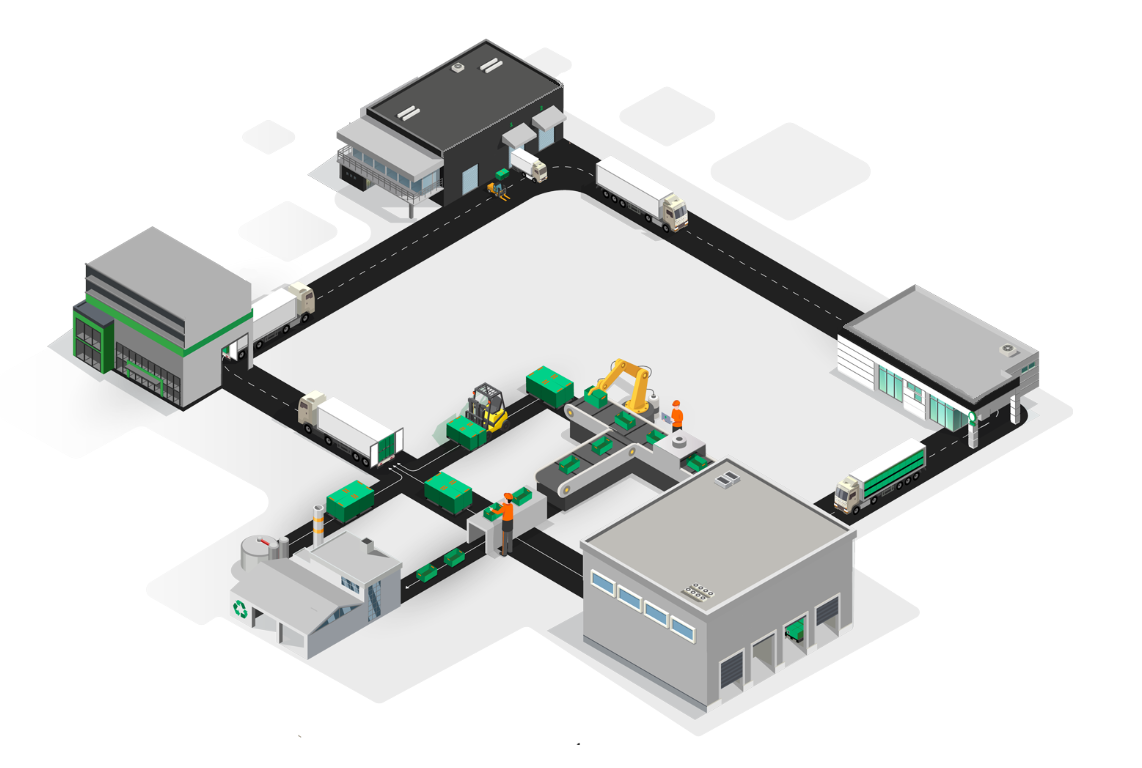
\includegraphics[width=8cm]{img/map.png}
    \centering
    \caption{Life cycle of company containers}
    \label{fig:covers}
\end{figure}

Currently the company has 13 warehouses strategically distributed in the country to facilitate the attention to their clients. In all the warehouses, there is an amount of containers/items of different types. These containers can be available to be used in a warehouse, they can stacked to be repaired in the same warehouse or they can be sent to a recycling center to make new ones. Each warehouse has a limited number of containers available for each type. However, it is possible that a large amount of containers are needed, so the company has the capacity to acquire more to supply the demand.

The main goal of the company is to transport the containers from warehouses to supermarkets. Currently, the company must optimize the planning of 2000 trips weekly. To this end, the company aims to develop an efficient search algorithm to plan the weekly allocation of a fleet of trucks in the different warehouses spread throughout the country. Due to physical and temporal constraints, the company aims to minimize the cost of transport generated by the trucks and the cost of stock in each of the warehouses. It must be taken into account that the amount of stock in the warehouses may be negative, so it means that the company must acquire them, so the cost of stock is directly associated with the price of items with negative stock.

This paper proposes a new SLAP proposal for balancing stocks taking into account that the problem can be modelled as a VRP, more specifically as an OVRP where the vehicle that transports the order does not return to its point of origin. To this end, A metaheurist search algorithm is proposed (GRASP). It searches for the first solution by applying a series of heuristics. Later, the local search is performed by applying a series of multi-target heuristics to filter the different solutions and choose the most optimized one.

\section*{Problem specification}

In this section, the problem specification posed by the company is provided for a better understanding of the proposed algorithm, highlighting the most relevant aspects. The main objective is to assign each trip to a warehouse, taking into account all the characteristics of each trip and warehouse. To this end, we seek to minimize the cost of transport and the extra cost of stock.  Minimizing the cost of the transport is relatively simple by obtaining the trip with the minimum cost. However, the cost of stock supposes a challenge, due to the fact that the stock of each container type must be balanced. To solve it, a multiobjective function must be determined by assigning weights to transport cost and stock cost to determine the fitness function. This function must maintains the transport cost stable while the stock in the warehouses is distributed homogeneously. Thus, the most important variables involved in the problem must be taken into account.

\begin{itemize}
  \item \textbf{Transport cost }(TC): is the cost associated with an order. This cost $tc$ is based on the distance between the starting point and the loading location, being proportional to the distance. This is taken into account when calculating the final cost in fitness function.
  \item \textbf{Extra stock cost }(SC): if an order composed of $N$ items to be delivered is loaded on a location where the current stock is less than the required, the remaining negative stock quantity must be replaced. Therefore, the cost of the stock will be proportional to the negative stock multiplied by the cost of replacing each of the items.
  \item \textbf{Delay of delivery }(DD): each of the possible locations associated with an order are located at a certain distance from the origin. Therefore, depending on the location chosen for loading the trip, a different delay will be assigned. This delay affects the amount of stock that is reduced from the loading station from the planned date to the real delivery date.
  \item \textbf{Single load point }(SLP): each order has a number of locations to which it can be uploaded. Each of these locations has a number of important decision features. An order can only be loaded at one location, with the constraint that all items needed in the order must be loaded at the same location. Thus, it is not allowed to load in different locations.
\end{itemize}

The problem is composed of a dataset (DS) which is based on the combination of three main elements that contains all necessary information to represent a problem instance (see Equation \ref{eq:Dataset}). Thus, each problem instance is composed of a set of orders (O) each of them representing a trip to transport items, a set of available warehouses (W) to load the items, and a set of prices (P) of each item.

\begin{equation}\label{eq:Dataset}
    \begin{aligned}
        DS = \{O, W, P\} \\
    \end{aligned}
\end{equation}

The set $O = \{o_1, o_2, \dots, o_N \}$ contains all information about the orders, where $N$ is the number of orders. Each order $o_i \in O$ is composed by three parameters $o_i =[D_{o_i},Ir_{o_i},W_{o_i}]$:
\begin{itemize}
    \item $D_{o_i}$ is the delivery date of $o_i$.
    \item $Ir_{o_i}$ contains the set of items to be loaded on the order (see Equation \ref{eq:OI}). Each element $ir_{o_{i}j} \in Ir_{o_i}$ represents the amount of items to be loaded.
    \begin{equation}\label{eq:OI}
        \begin{aligned}
            Ir_{o_{i}} = \{ ir_{o_{i}1}, ir_{o_{i}2} \dots, ir_{o_{i}P} \} \\
        \end{aligned}
    \end{equation}
    \item $W_{o_i}$ is a set of possible warehouses where order $o_i$ can load all required items (see Equation \ref{eq:OW}).
    \begin{equation} \label{eq:OW}
        \begin{aligned}
            W_{o_i} = \{ W_{o_{i}1}, W_{o_{i}1}, \dots W_{o_{i}Q} \}\\
        \end{aligned}
    \end{equation}
    Each element $W_{o_{i}j}$ is formed by three values:
    \begin{itemize}
        \item $ava_{o_{i}j}$ represents the availability of platform $j$ to load all items of order $o_i$. Thus, $ava_{o_{i}j}=1$  means the warehouse is available, and $ava_{o_{i}j}=0$ otherwise.
        \item $pr_{o_{i}j}$ contains the transport cost of order $o_i$ from platform $j$. If $ava_{o_{i}j}=0$ this value is null.
        \item $dl_{o_{i}j}$ is the delay to load the order $o_i$ from platform $j$. If $ava_{o_{i}j}=0$ this value is null.
    \end{itemize}
\end{itemize}

To control the amount of stock at the beginning of each week, the company provides a tridimentional matrix with the current status of each warehouse $W$ (see Equation \ref{eq:W}).
\begin{equation}
    \begin{aligned}\label{eq:W}
        W = \{w_1, w_2, w_3, \dots w_P \}\\
    \end{aligned}
\end{equation}
where each $wst_i \in W$ is composed of a bidirectional matrix (item x date of week ). Due to the model of the company, it is allowed to generate negative stock in the warehouses associated to an order $wst_{ijk} \in \mathbb{N} $. This is allowed because each of the logistic centers (warehouse) can replace the lack of containers by shipping them.

Finally, $P$ is the set of unitary price for each items/article (see Equation \ref{eq:P}).

\begin{equation}
    \begin{aligned}\label{eq:P}
        P = \{p_1, p_2, p_3, \dots, p_i, \dots p_P \}\\
    \end{aligned}
\end{equation}


\section*{Solving techniques}

This section aims to explain the current algorithm working on the company, pointing out the structure and specifications of the implemented greedy algorithm, as well as the characteristics that make it up. Next, the proposed GRASP algorithm, local search and several improvements are detailed.

\subsection*{Greedy algorithm }
Currently, the objective of company is the planning of weekly orders based on the demand requested by customers taking into account the available stock expected for each day of the week. The company has developed its own algorithm to obtain an optimized solution based on a greedy technique with a post-processing phase.
The stock available in each article model in a week is obtained from a weekly load plan. This stock is obtained from the sum of the remaining containers from the previous week, the containers that have been successfully restored and those obtained by shipments, among others. The greedy algorithm has additional constraints posed from the perspective of the customer, warehouses and geographical areas, in addition to other factors:

\begin{itemize}
    \item A certain number of clients only allow loading in a certain warehouse due to distance and comfort factors.
    \item The zone of influence or geographical area has a higher priority in the assignment of orders by each warehouse.
    \item The loading of an order is restricted to the type of items it contains, so there are certain warehouse that do not serve a particular item.
    \item The warehouses or loading centres have independent delays for each product at different times of the year, as the quantity of products (fruit, vegetables, fishes) is not constant throughout the year.
\end{itemize}

These constraints make the generated search tree too large to be addressed in one go. Therefore, the current algorithm developed by the company is split into several layers, which are put together in a post-processing step.

 Firstly, the algorithm performs an ordering according to priorities. It uses a heuristic called closeness centrality applied to network theory. This measure allows us to obtain a measure of centrality of a transport network by adding the length of the paths between the different nodes, obtaining the central nodes as those that are closer to the other nodes. Later, the orders are classified according to the article with greater portion of the order, assigning all the available stocks of the nearest warehouses by this article model.

In the second layer, there are unassigned orders to a warehouse because they have failed to meet any of the restrictions of the first layer. These remaining orders are reordered with the centrality closeness heuristics to assign them to less central warehouses with larger stock. The orders that have not been assigned can be renegotiated with the customers to improve the response of the warehouse system or make up for the lack of stock by manufacturing containers needed to meet the customers' needs. However, after this second layer, there may be unassigned orders which are assigned to the most optimal warehouse in a post processing. These are marked, so that an expert human must review them, looking for combinations that improve the cost of global transport without increasing the extra cost of stock to manufacture containers.
The constraints that are joined in the greedy algorithm by layers only take into account the cost that generates the transport and the requests of the clients, forcing an expert to review all the trips to be able to obtain a better solution for the company.

\subsection*{GRASP}

Taking into account the structure of the above greedy method and its drawbacks to obtain an good solution, a GRASP algorithm is developed to obtain a balanced solution in terms of travel cost and stock balance. To do this, we focus on obtaining an efficient solution and keeping the stock as balanced as possible among the warehouses.

\begin{algorithm}[H]
    \caption{GRASP}
    \label{alg:GRASP}
    \begin{algorithmic}[1] \label{code:grasp}
        \STATE \textit{input: } All orders $O$, All stock matrix $W$, Item price vector $P$, Size of LR list $n$
        \STATE \textit{output: } Optimized solution $s^*$
        \STATE $i \longleftarrow 0 $
        \STATE $ t \longleftarrow [1,2,3,\dots,|O|]$
        \STATE \textbf{while} empty($t$) \textbf{do}: \label{1order}
        \STATE \quad \textbf{if} sort-criterion(i) \textbf{then}: \label{sort-criterion}
        \STATE \quad \quad swap( $ o_{i-1}$ , $ o_{i} $ )
        \STATE \quad \quad $t \longleftarrow t \setminus i$
        \STATE \quad \quad $i \longleftarrow i + 1$
        \STATE \quad $\textbf{end if}$
        \STATE $\textbf{end while}$ \label{2order}
        \STATE
        \STATE $s \longleftarrow [\quad] $
        \STATE $LR \longleftarrow [o_1,\dots,o_n]$
        \STATE \textbf{while } $|s| \neq |LR|$ \textbf{do}:\label{1grasp}
        \STATE \quad $j \longleftarrow 0 $
        \STATE \quad $lcr \longleftarrow [\quad]$
        \STATE \quad \textbf{while } $j < |LR|$ \textbf{do}:
        \STATE \quad \quad $lcr \longleftarrow lcr \cup \textbf{LocalSearch}(LR_j,P,\alpha,|LR|)$
        \STATE \quad \quad $j \longleftarrow j + 1$
        \STATE \quad $\textbf{end while}$
        \STATE \quad $s \longleftarrow s \cup lcr*$
        \STATE \quad $LCR \longleftarrow LR \setminus lcr*$
        \STATE \quad $LCR \longleftarrow LR \cup  o_{n+1} $
        \STATE \quad $n \longleftarrow n +  1 $
        \STATE $\textbf{end while}$\label{2grasp}
        \STATE $\textbf{return } s^*$
    \end{algorithmic}
\end{algorithm}


The proposed algorithm \ref{code:grasp} is based on two steps. First, the list of orders is sorted to improve the response of the algorithm (from lines \ref{1order} to \ref{2order}). This assumption is based on the idea of constrainedness, analyzing the most restrictive orders first in order to give the algorithm more decision power in the final iterations. And secondly, the iterative part of GRASP (from line \ref{1grasp} to \ref{2grasp}) obtains a fraction of the size of the list of requests (LR). This list contains the algorithm's candidates to assign a warehouse. Then. a local search is generated in which the best warehouse is obtained. Once we have the best warehouses for all the trips, we select the warehouse with the lowest cost, eliminating the order from the LR list and adding the next one from the sorting list.

\subsubsection*{LR ordering}
The sorting of the LR list is carried out to give more flexibility and to test the behaviour of the algorithm with different inputs. This pre-processing auto-allocates all the trips that have only one available warehouse due to availability or customer's restrictions.

This type of ordering is modular for easier testing. For this purpose, a sorting algorithm is developed based on a criterion (see Line \ref{sort-criterion}. Once all the values in the list are correctly sorted, the list with these values is returned.


\begin{itemize}
    \item \textbf{Sort by number of warehouses (Model 1) :} the list is ordered by the number of possible warehouses, that is, the first order in the list will have less warehouses, allowing the algorithm to assign them with less number of decisions to make (constrainedness).
    \begin{itemize}
        \item \textbf{Sort by number of warehouses and items (Model 2) :} Among the trips ordered by warehouses and with the same value, they are ordered by the least number of items required for the trip.
        \item \textbf{Sort by number of warehouses and delay (Model 3) :} Among the trips ordered by warehouse, they are ordered according to the number of days of delay in that order. This is because the more days of delay there are, the more blocked stock remains during the week.
    \end{itemize}
    \item \textbf{Sort by Delay and Items (Model 4) :} In this case, orders are classified by the sum of the delays of all their warehouses and by the amount of items required for the trip.

    \item \textbf{Sort by warehouses plus standardized delay and items (Model 5) :} this sorting is carried out by mixing the three criteria previously defined. To do this, we add the standardization of the delay and the number of warehouses and then order by the number of items.
    \item \textbf{Sort by number of weight warehouses and delay (Model 6) :} This sorting is based on the previous one by adding a beta weight to the delay. Then, the sorting is done by number of items.
\end{itemize}

After carrying out some tests to verify the viability of all sorting types, it was found that sorting by number of warehouses, more specifically, sorting by number of warehouses and items gave the best results without negatively affecting time or computer costs.

\subsection*{Local search}

Once we have the order list sorted, we iterate it to execute a local search on each order in order to obtain the best assignation. This local search is based on obtaining the objective function for each of the possible warehouses in a trip, by generating a list of values for each warehouse. Once this list is obtained, we will obtain the minimum value of it and the select warehouse is assigned to the trip.

\begin{algorithm}[H] \label{code:LocalSearch}
    \caption{Local Search}
    \begin{algorithmic}[1]
        \STATE \textit{input: } A order $o$, List of item price $P$, Alpha value for objetive funtion $\alpha$, Length of LR list $n$
        \STATE \textit{output: }  Best choice of warehouse $Q^*$
        \STATE  $Q \longleftarrow [\quad]$
        \STATE  $I \longleftarrow Ir_{o}$
        \STATE  $M \longleftarrow W_{o}$
        \STATE  \textbf{For} $j$ \textbf{in} $\{ 0,\dots,|M|\}$:
        \STATE  \quad $Cs \longleftarrow 0$
        \STATE  \quad $Ct \longleftarrow \textbf{getTransportCost}(M_j) $ \label{eq:ct}
        \STATE  \quad \textbf{For} $i$ \textbf{in} $\{ 0,\dots,|I|\}$:
        \STATE  \quad \quad $Cs_i \longleftarrow P_i * \sum_{k=D_{o}}^{|wst_{ij}|} wst_{ijk}\; |\; wst_{ijk} < 0 $ \label{eq:cs}
        \STATE  \quad \quad $Cs \longleftarrow Cs + Cs_i$
        \STATE  \quad  $\textbf{end for}$
        \STATE  \quad $Q_j \longleftarrow \alpha * Ct + (1 - \alpha) * Cs$ \label{eq:fitness}
        \STATE  \quad $Q \longleftarrow Q \cup Q_j$ \label{eq:fitness}
        \STATE  \quad $F_{\alpha}  \longleftarrow \frac{1-\alpha}{n}$ \label{eq:fitness}
        \STATE  \quad \textbf{if} $\sum Cs < 0$ \textbf{then}:
        \STATE  \quad \quad $\alpha \longleftarrow \alpha + F_{\alpha}$
        \STATE  \quad $\textbf{else:}$
        \STATE  \quad \quad $\alpha \longleftarrow \alpha - F_{\alpha}$
        \STATE  \quad $\textbf{end if}$
        \STATE  $\textbf{end for}$
         \STATE  $Q^* \longleftarrow \textbf{getBest}(Q)$
        \STATE  $\textbf{return } Q^*$
    \end{algorithmic}
\end{algorithm}

In each iteration, one of the orders in the LR list is analyzed and the objective function is calculated with all the items that compose the order and the possible warehouses to obtain the best one. The objective function is based on calculating the cost of transport and the cost of stock and weighting them with an alpha value to give more weight to the cost of transport which generates more costs (see Line \ref{eq:fitness}).
The transportation cost of a trip is obtained by adding the price of traveling to a warehouse of each order (see Line \ref{eq:ct}). The cost of the stock is obtained by subtracting the quantity of an article required in a warehouse in a certain day, multiplying by its price in the case that the stock is negative. If the stock remains positive the cost of the stock will be zero (see Line \ref{eq:cs}). The warehouse assignments for each trip is stored and the best assignment is selected.

\subsection*{Improvements}
During the development of the algorithm, several issues appear that negatively affect the optimality of the solution. To overcome these issues, solutions are composed independently of the main code to avoid problems in the efficiency of the algorithm.

The first issue is observed when several GRASP iterations are performed over the same sorting mode, so the algorithm returns identical results because the sorting is so specific that there is no option for certain trips to be sorted differently, i.e. a certain trip in a sorting mode always ends up in the same position in the list. In order to solve this problem, a \textit{shuffle} method is generated which exchanges those trips that have more similar characteristics depending on the chosen sorting mode.

The next issue is related to obtaining an optimized solution. Due to the constant update of the stock matrices during the iterations of the algorithm, it is observed that in problems in which the quantity of stock of the orders is higher than the served by the warehouses, it proves a polarization of the objective function generating an unbalance in the allocation of the warehouses. To overcome this issue, a \textit{alpha scheduler} is generated to update the target function in each of the iterations to avoid this polarization. An alpha parameter is entered in the target function, which increases or decreases its value depending on the assignment in each of the iterations. In case the remaining stock in the selected platform for that trip is positive, alpha grows to give more importance to the transport cost. Otherwise, if the value of the platform stock is negative, the alpha parameter decreases giving more influence to the stock cost.

\section*{Evaluation}

This section presents the results obtained from the comparison of the greedy algorithm implemented by the company and the proposed GRASP algorithm. To this end, several case studies were carried out and the results were split in both objectives: transportation cost and stock balance. The runtime is not included in the next tables due to the fact that the Greedy algorithm had a worse behaviour than the proposed GRASP algorithms in all instances. In average, the runtime for the Greedy algorithm was around 20 minutes for solving each instance, meanwhile the GRASP algorithm took around 50 seconds to solve it. All instances had a different complexity due to the fact that they represents real instances corresponding to different weeks of June and July, 2020. In average, each instance is composed on 1800 trips, each of them involving 5-10 warehouses.

\begin{table}[H]
    \centering
    \begin{tabular}{|c|c|c|}
    \hline
    \textbf{Date}   & \textbf{Greedy} & \textbf{GRASP} \\ \hline
    \textbf{Week 1} & 214             & 233            \\ \hline
    \textbf{Week 2} & 217             & 244            \\ \hline
    \textbf{Week 3} & 219             & 242            \\ \hline
    \textbf{Week 4} & 216             & 235            \\ \hline
    \end{tabular}
    \caption{Transportation cost}
    \label{tab:georesultados}
\end{table}

 Table \ref{tab:georesultados} shows the transportation cost of 4 different instances. It can be observed that the transportation cost is lower in the greedy algorithm than the GRASP algorithm. This is due to the fact that the greedy algorithm is developed to obtain the lowest transportation cost by using the centrality heuristic. However it does not tale into account the stock balance.


\begin{figure}[H]
    \begin{subfigure}{.5\textwidth}
      \centering
      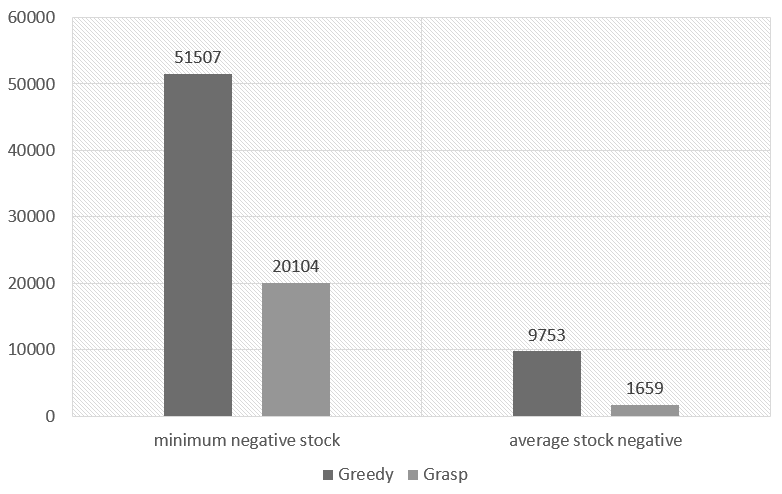
\includegraphics[width=\linewidth]{img/week1-stock.png}
      \caption{Week 1 extra stock cost}
      \label{fig:week1}
    \end{subfigure}
    \begin{subfigure}{.5\textwidth}
      \centering
      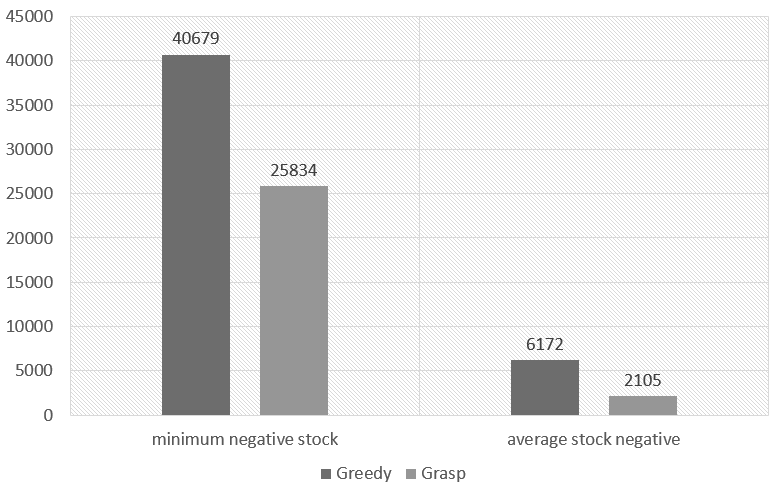
\includegraphics[width=\linewidth]{img/week2-stock.png}
      \caption{Week 2 extra stock cost}
      \label{fig:week2}
    \end{subfigure}
    \caption{Extra stock cost}
    \label{fig:stock}
\end{figure}


To correctly evaluate the concentration of remaining stock in the warehouses, two metrics are generated. The first one obtains the most negative value in all the warehouses (see Figure \ref{fig:week1}). This allows us to determine when the algorithm is wrongly balancing the stock and to be able to compare the stock concentration between the two algorithms. The second metric is based on obtaining the average of negative stock of all warehouses (see Figure \ref{fig:week2}). The results obtained by this metric help us to have a more global vision of the stock balancing by the two algorithms. The results of the GRASP algorithm regarding the amount of remaining stock in the different weeks indicate that the load balancing was being effective, with up to 82\% improvement in negative average stock and 60\% in negative minimum stock.


\section*{Conclusions and future work}


Transport companies need to optimize their logistics infrastructures and strategies to be more efficient in a more competitive word. The proposed problem tries to merge two different problems, the warehouse stock management problem and the routing problem to minimize both the negative stock and transport cost. To this end, a GRASP-based metaheuristic has been developed to improve the greedy algorithm that is currently managed by the company. The results on several case studies show that although the greedy algorithm had a better behaviour in the transport cost, due to it is specially guided by a heuristic. However the proposed GRASP algorithm overcomes the results obtained by the greedy algorithm in the stock balancing, improving the negative average stock up to 82\%.

In further works, we will improve the proposed algorithm by combining the proposed GRASP algorithm with a genetic algorithm (GA). Thus, the solutions obtained by the GRASP algorithm will participate as a subset of the initial population for the genetic algorithm. It could improve the quality of the solutions due to the high capability of the GA to combine previous solutions and avoid trapping in local optima.

%\section*{Acknowledgements}
%The paper has been partially supported by the Spanish research project TIN2016-80856-R.

\bibliography{bib}
\bibliographystyle{aaai}
\end{document}
